% !TEX root = ../WassersteinDual.tex
% better to integrate it there?
%\section{Numerical Experiments}\label{sec:numericalresults}

%%%%%%%%%%%%%%%%%%%%%%%%%%%%%%%%%%%%%%%%%%%%
\subsection{Smoothing and Stabilization of the WBP}
\label{sec:wassbarprob}
We make the claim in this section that smoothing the WBP is not only beneficial computationally, but may also yield more stable computations. Of central importance in this discussion is the fact that the WBP can be cast as a LP of $Nn^2+n$ variables and $2Nn$ constraints, and thus solved \emph{exactly} for small $n$ and $N$:
\begin{equation}\begin{aligned}\label{eq-WBP-simplex}
	\min_{X_1,\cdots,X_N,p}& \sum_{k=1}^N \la_k  \dotp{X_k}{M}\\
	\text{s.t. } & X_k \in \RR^{n\times n}_+, \forall k\leq N; p\in\Sigma_n,\\
	& X_k^T \ones_n = \q_k, \forall k\leq N,\\
	 & X_1 \ones_n = \dots = X_N \ones_n= p.
\end{aligned}\end{equation}
Given couplings $X_1^\star,\cdots,X_N^\star$ which are optimal solutions to Eq.\eqref{eq-WBP-simplex}, the solution to the WBP is equal to the marginal common to all those couplings: $p^\star=X_k^\star \ones_n$ for any $k\leq N$. For small $N$ and $n$, this problem is tractable, but it can be surprisingly ill-posed as we see next.

Indeed, it is also known that the $2$-Wasserstein mean of two univariate (continuous) Gaussian densities of mean and standard deviation $(\mu_1,\sigma_1)$ and $(\mu_2,\sigma_2)$ respectively is a Gaussian of mean $(\mu_1+\mu_2)/2$ and standard deviation $(\sigma_1+\sigma_2)/2$~\cite[\S6.3]{Carlier_wasserstein_barycenter}. This fact is illustrated in the top-left plot of Figure~\ref{fig:smoothvsnonsmooth} where we display the average Wasserstein average $\Ncal(0,5/8)$ of the two densities $\Ncal(2,1)$ and $\Ncal(-2,1/4)$. That plot is obtained by using smoothed spline interpolations of a uniformly spaced grid of $100$ values, as can be better observed in the top-right (stair) plot, where the discrete evaluations of these densities are respectively denoted $p_W$, $q_1$ and $q_2$.

Naturally, one would expect the barycenter of $q_1$ and $q_2$ to be close, in some sense, to the discretized histogram $p_W$ of their true barycenter. Histogram $p^\star$, displayed in the bottom-left plot, is the exact optimal solution of Eq.~\eqref{eq-WBP-simplex}, computed with the simplex method. That WBP reduces to a linear program of $2\times 100^2$ variables and $300$ constraints. We observe that $W_2^2(p^\star,q_1)+W_2^2(p^\star,q_2)=0.5833950$ whereas  $W_2^2(p_W,q_1)+W_2^2(p_W,q_2)=0.5834070$. The solution obtained with the simplex has, indeed, a smaller objective than the discretized version of the true barycenter.

The bottom-right plot displays the solution of the \emph{smoothed} Wasserstein barycenter problem (with smoothing parameter $\gamma=\frac{1}{100}$ and a ground cost $M$ that has been re-scaled to have a median value of $1$). The objective value for that smoothed approximation is $0.5834597$.

This numerical experiment does not contradict the fact that the discretized barycenter $p^\star$ converges to the continuous barycenter as the grid size tends to zero, as shown in~\cite{Carlier-NumericsBarycenters}. This observation illustrates however that, because it is defined as the $\argmin$ of a linear program, the true Wasserstein barycenter may be extremely unstable, even for such a simple problem and for large $n$ as illustrated in Figure~\ref{fig:smoothvsnonsmooth2}. Regularizing the Wasserstein distances has thus the added benefit of smoothing the resulting solution of the Wasserstein barycenter problem, and that of mitigating low sample size effects.

The choice of the parameter $\gamma$ is application-dependent, but it should scale with the typical distance between sampling locations (e.g. the grid step size). Note that choosing too small $\gamma$ not only leads to slower convergence of our algorithm, but also leads to numerical instabilities and can ultimately breaks the convergence.  

% ------> Version avec une seule figure, mises côte à côte. je trouve que les fonts sont trop petites.
%
% \begin{figure}[ht]
% 	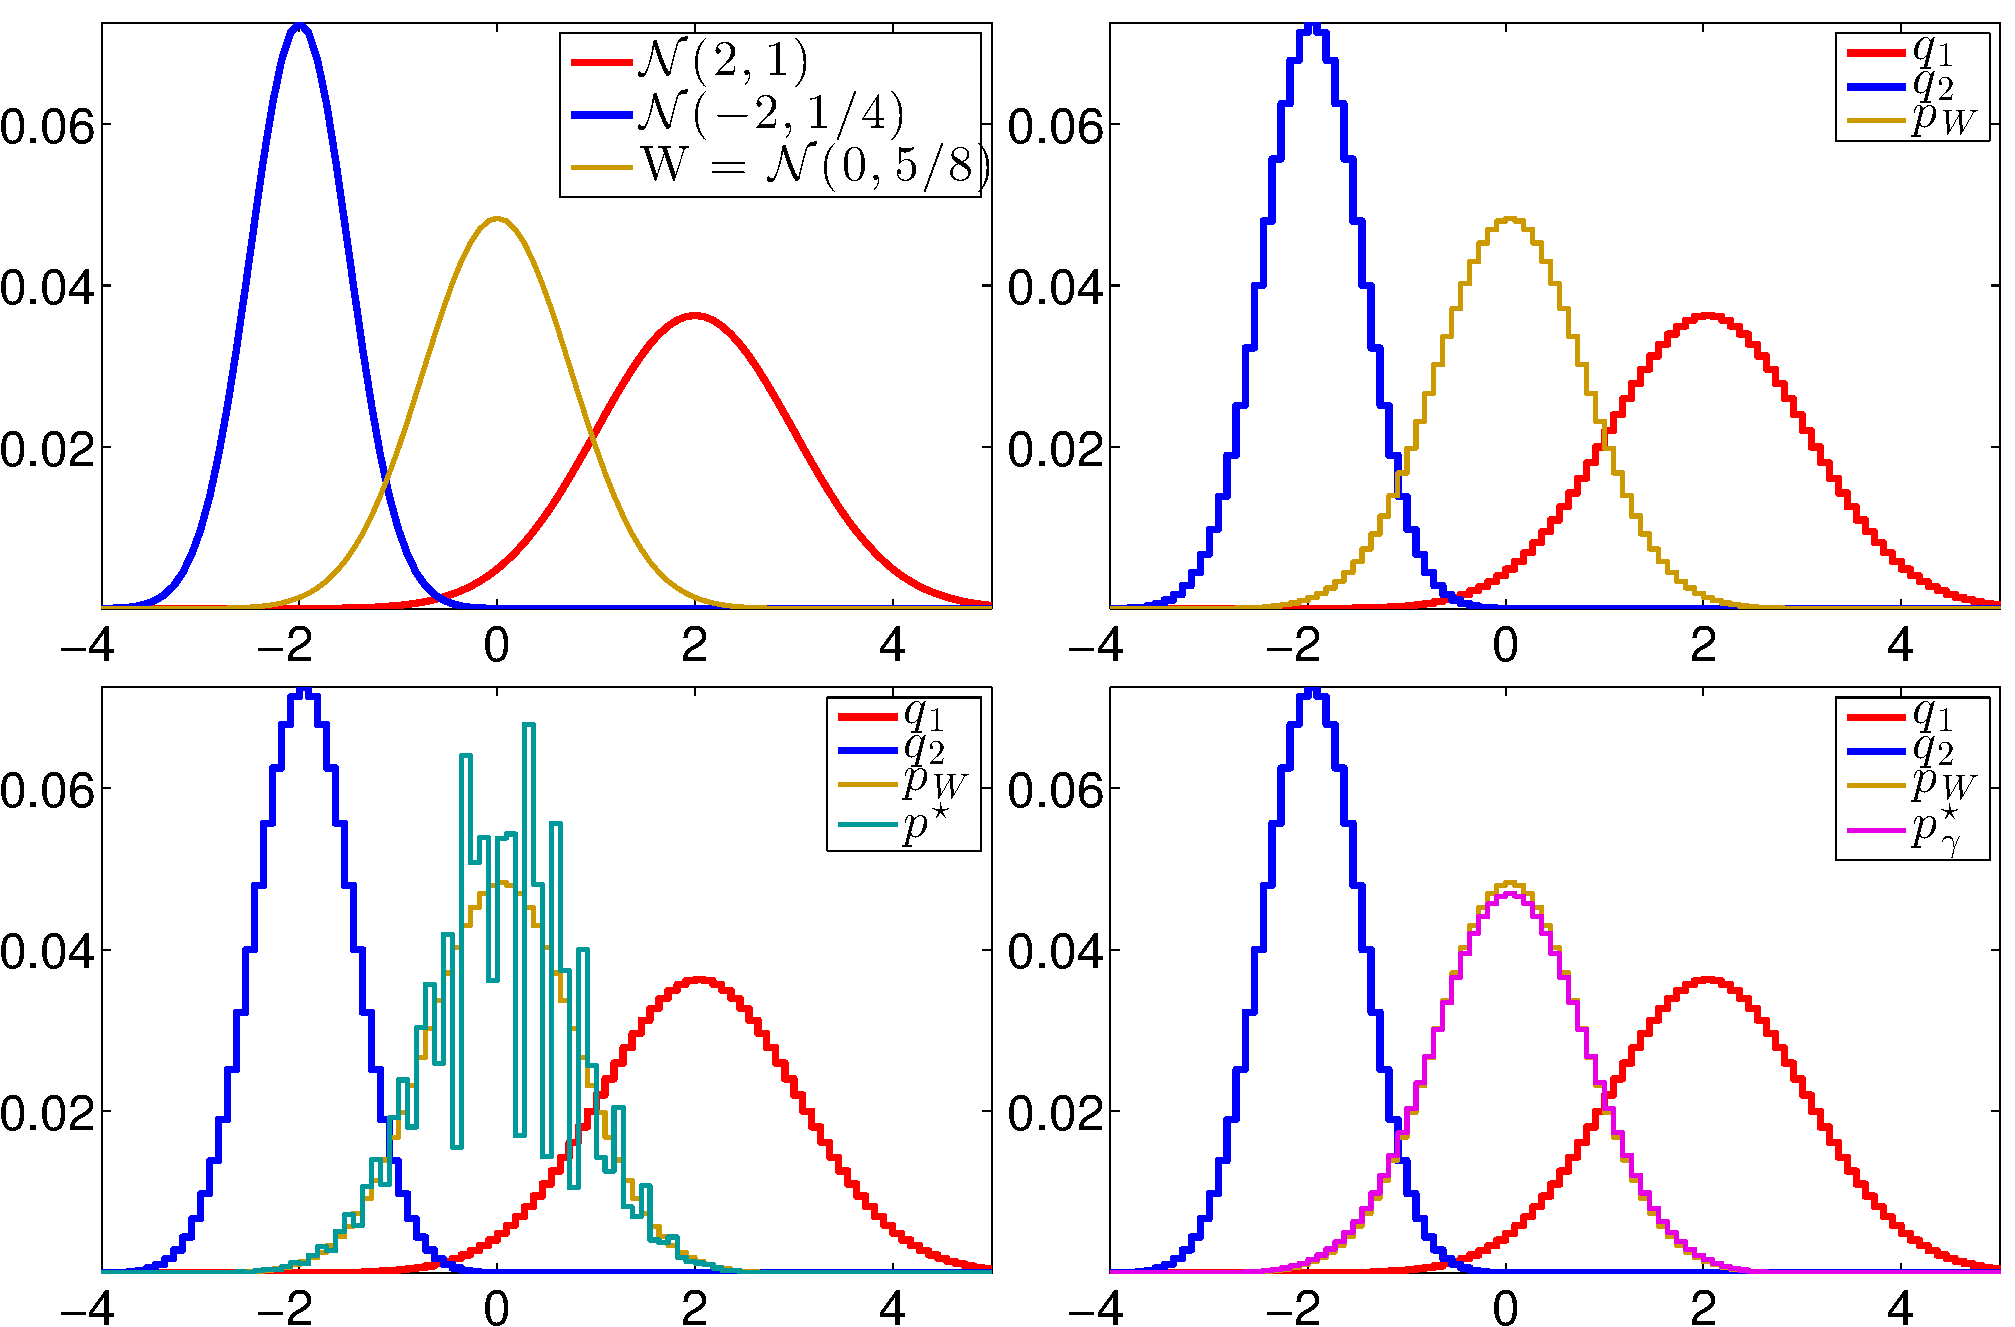
\includegraphics[width=.5\linewidth]{smoothvsnonsmooth.pdf}    
% 	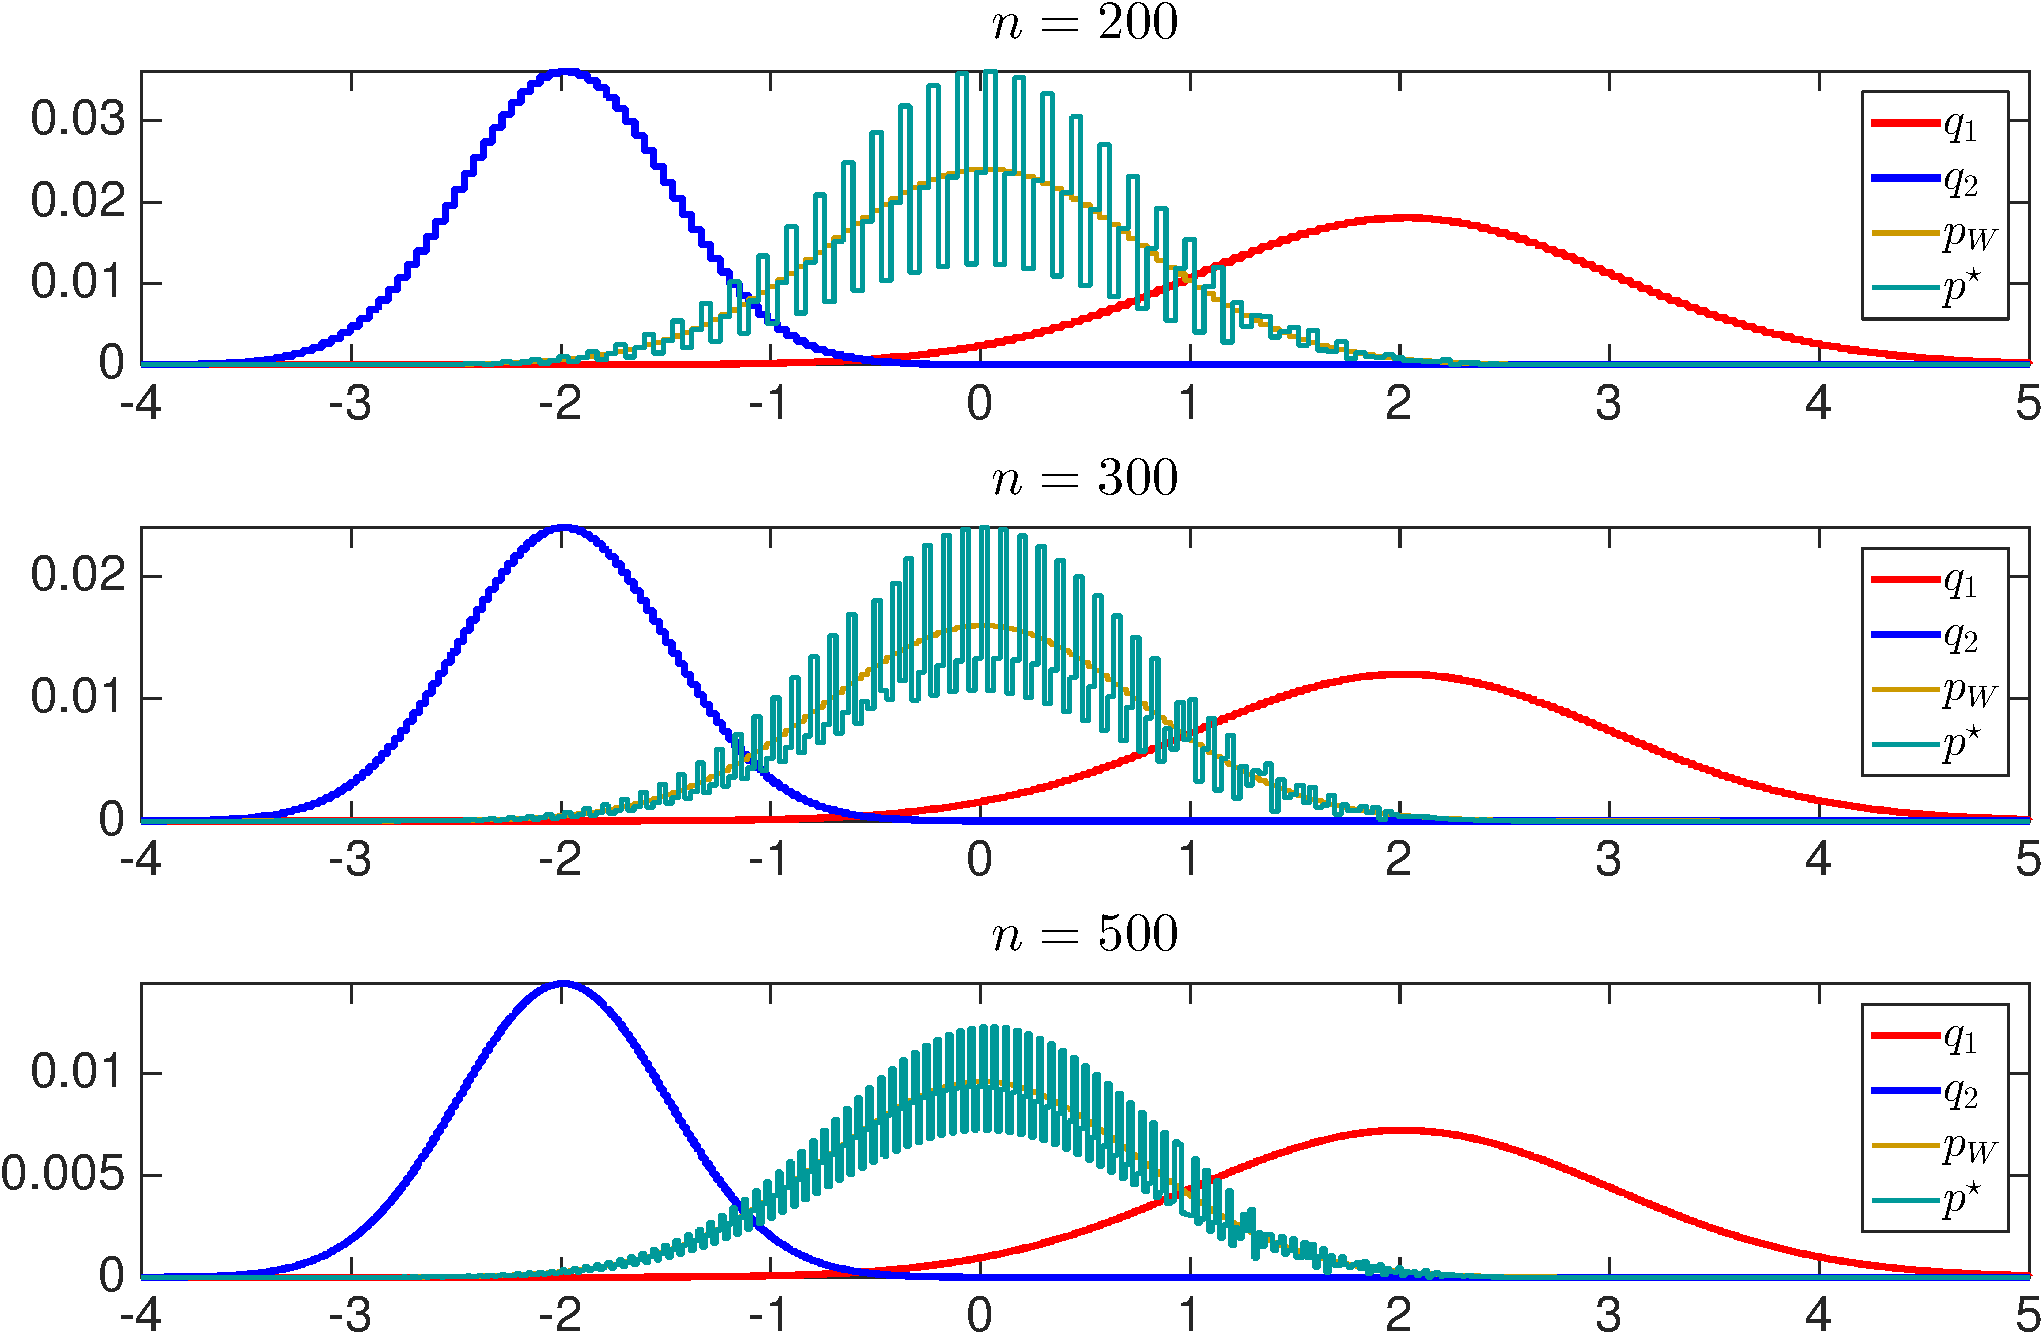
\includegraphics[width=.5\linewidth]{nonsmoothsnot_conv.pdf}
% 	\caption{(top-left) two Gaussian densities and their barycenter (top middle) same densities, discretized (bottom left) discretization of the true barycenter \emph{vs.} the optimum of Eq.~\ref{eq-WBP-simplex} (bottom middle) barycenter computed with our smoothing approach. (right) Plots of the exact barycenters for varying grid size $n$}\label{fig:smoothvsnonsmooth}
% \end{figure}

\begin{figure}[ht]
	\centering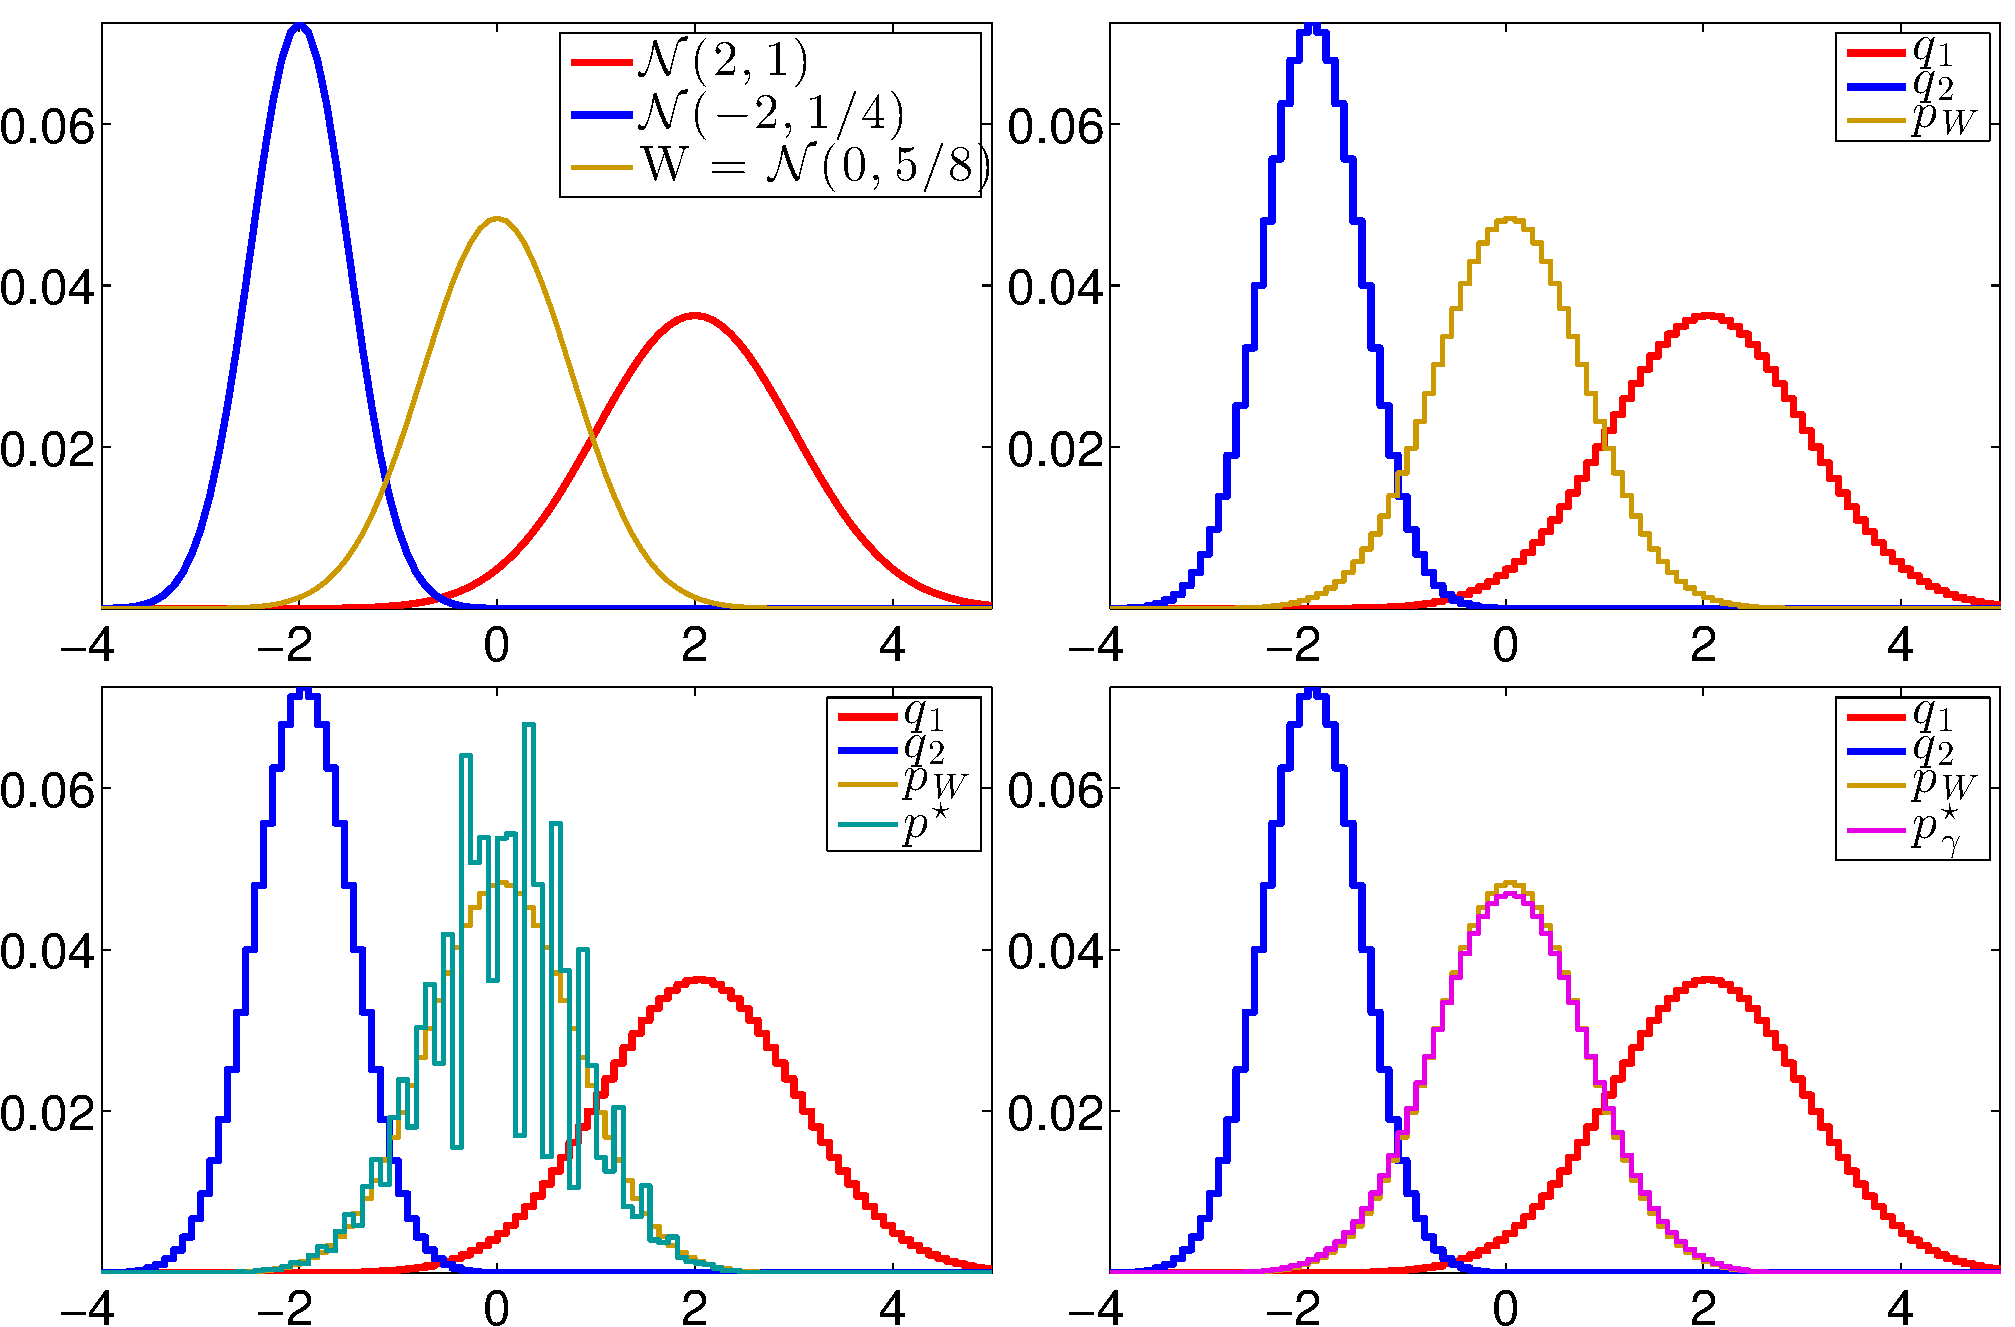
\includegraphics[width=.75\columnwidth]{smoothvsnonsmooth.pdf}    
	\caption{(top-left) two Gaussian densities and their barycenter (top right) same densities, discretized (bottom left) discretization of the true barycenter \emph{vs.} the optimum of Equation~\ref{eq-WBP-simplex} (bottom right) barycenter computed with our smoothing approach. }\label{fig:smoothvsnonsmooth}
\end{figure}

\begin{figure}[ht]
\centering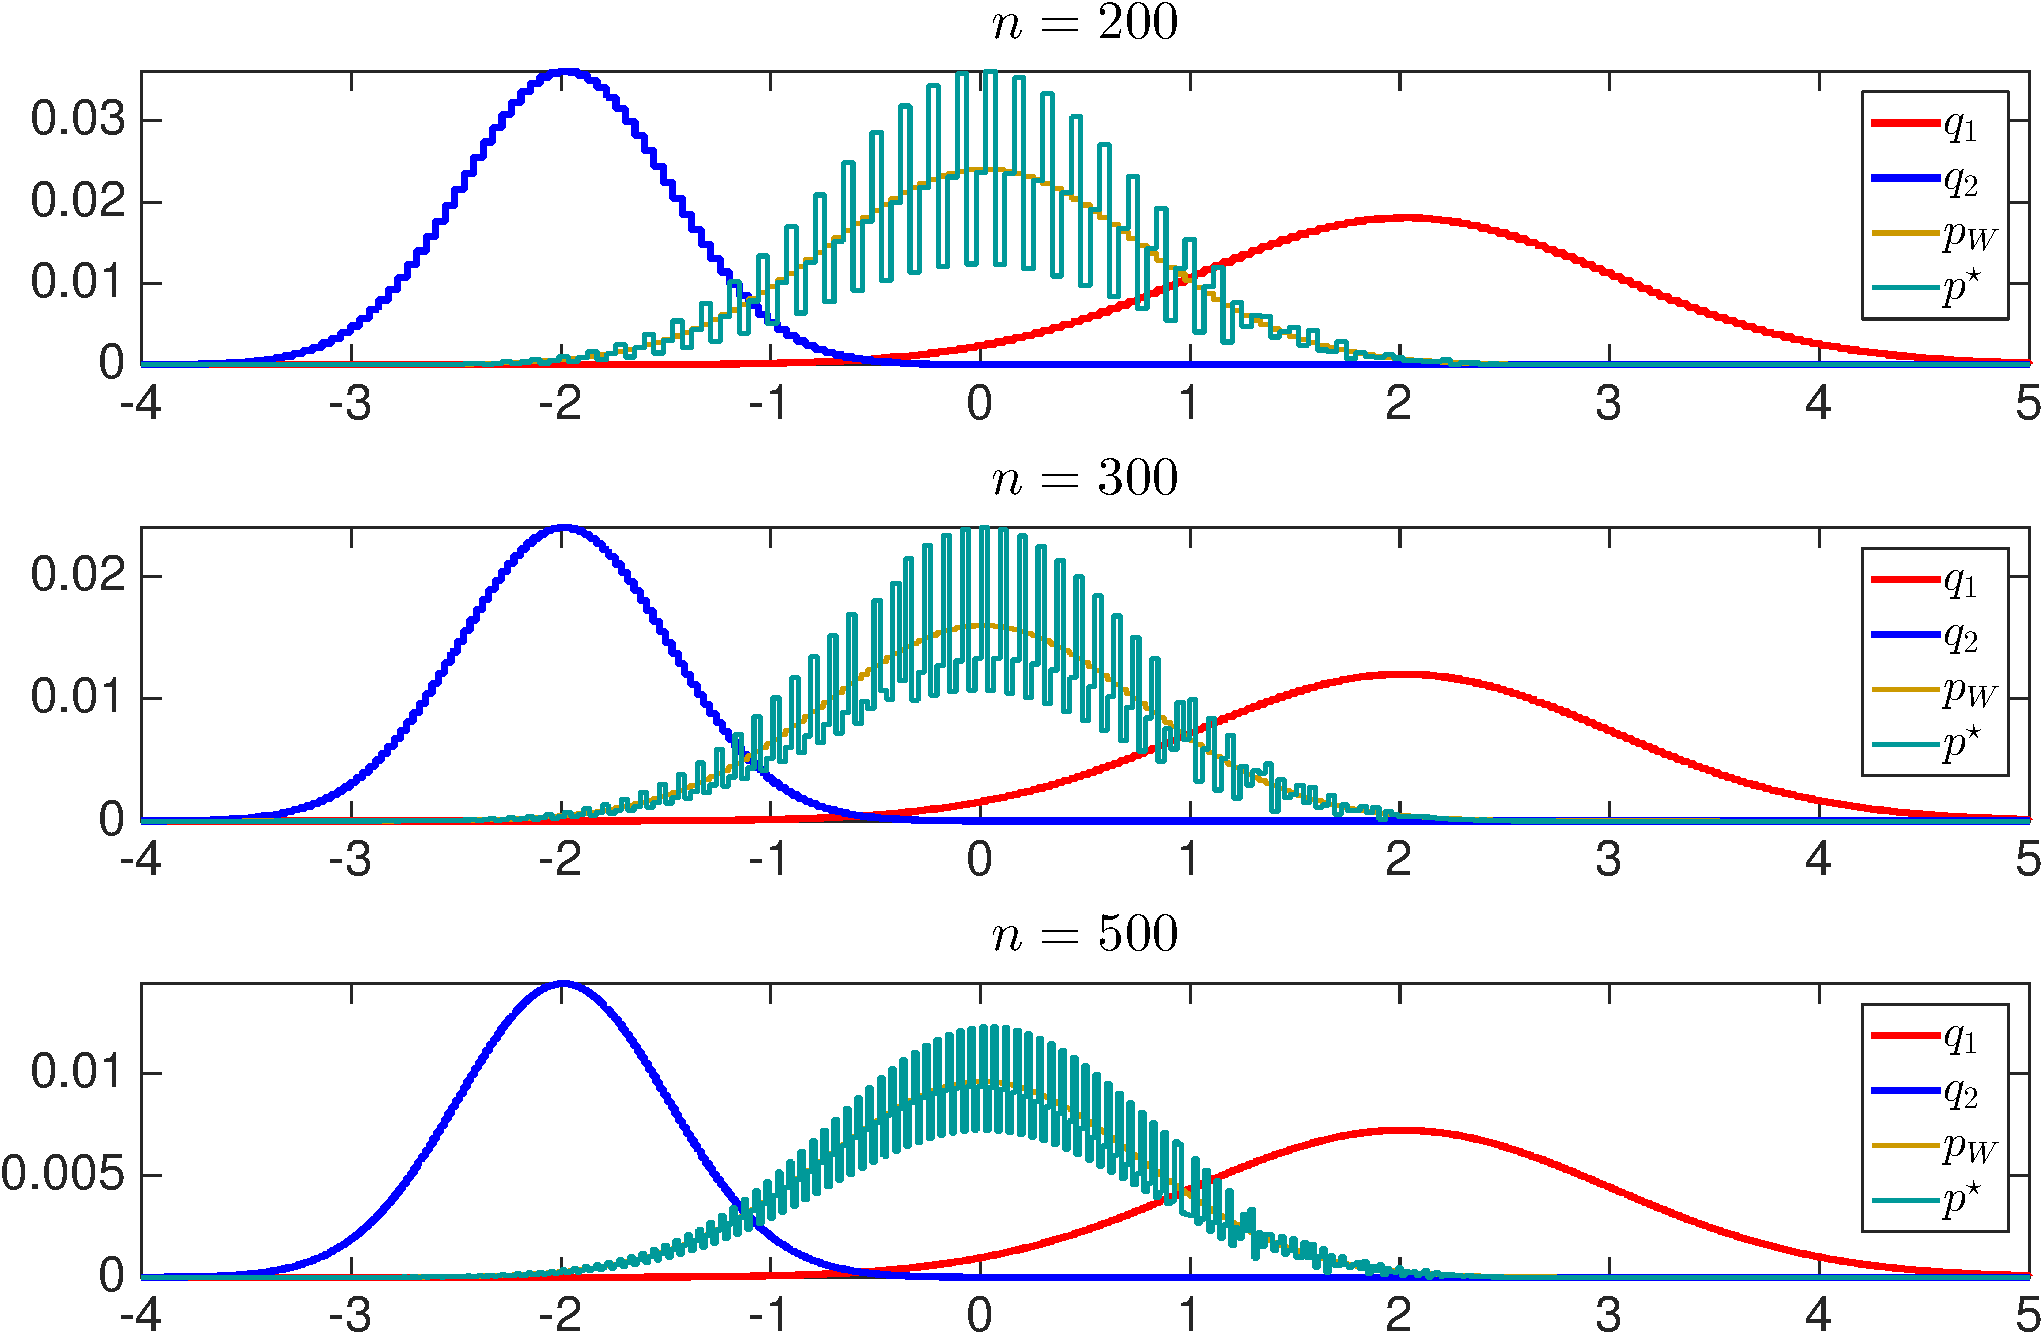
\includegraphics[width=.75\columnwidth]{nonsmoothsnot_conv.pdf}    
\caption{Plots of the exact barycenters for varying grid size $n$.}
\label{fig:smoothvsnonsmooth2}
\end{figure}

%%%%%%%%%%%%%%%%%%%%%%%%%%%%%%%%%%%%%%%%%%%%
\subsection{Performance on the Wasserstein Barycenter Problem}
We compare in this section the behavior of the smooth dual approach presented in this paper with that of (i) the smooth primal approach of~\cite{cuturi2014fast}, (ii) the dual approach of \cite{Carlier-NumericsBarycenters}, and (iii) the Bregman iterative projections approach of \cite{DBLP:journals/siamsc/BenamouCCNP15}. We compare these methods on the simple task of computing the Wasserstein barycenter of $12$ histograms laid out on the $100\times100$ grid, as previously introduced in \cite[\S3.2]{DBLP:journals/siamsc/BenamouCCNP15}. We outline briefly all four methods below, and follow by presenting numerical results.

% \begin{figure}[h!]
% \centering\includegraphics[width=\columnwidth]{mymixture.png}
% 	\caption{12 measures, truncated mixtures of Gaussians, used in our benchmark. Convergence speed results displayed in Figure~\ref{fig:costs3} and barycenters obtained in~\ref{fig:bar}}.\label{fig:mix}
% \end{figure}


\begin{figure}[h]
	\centering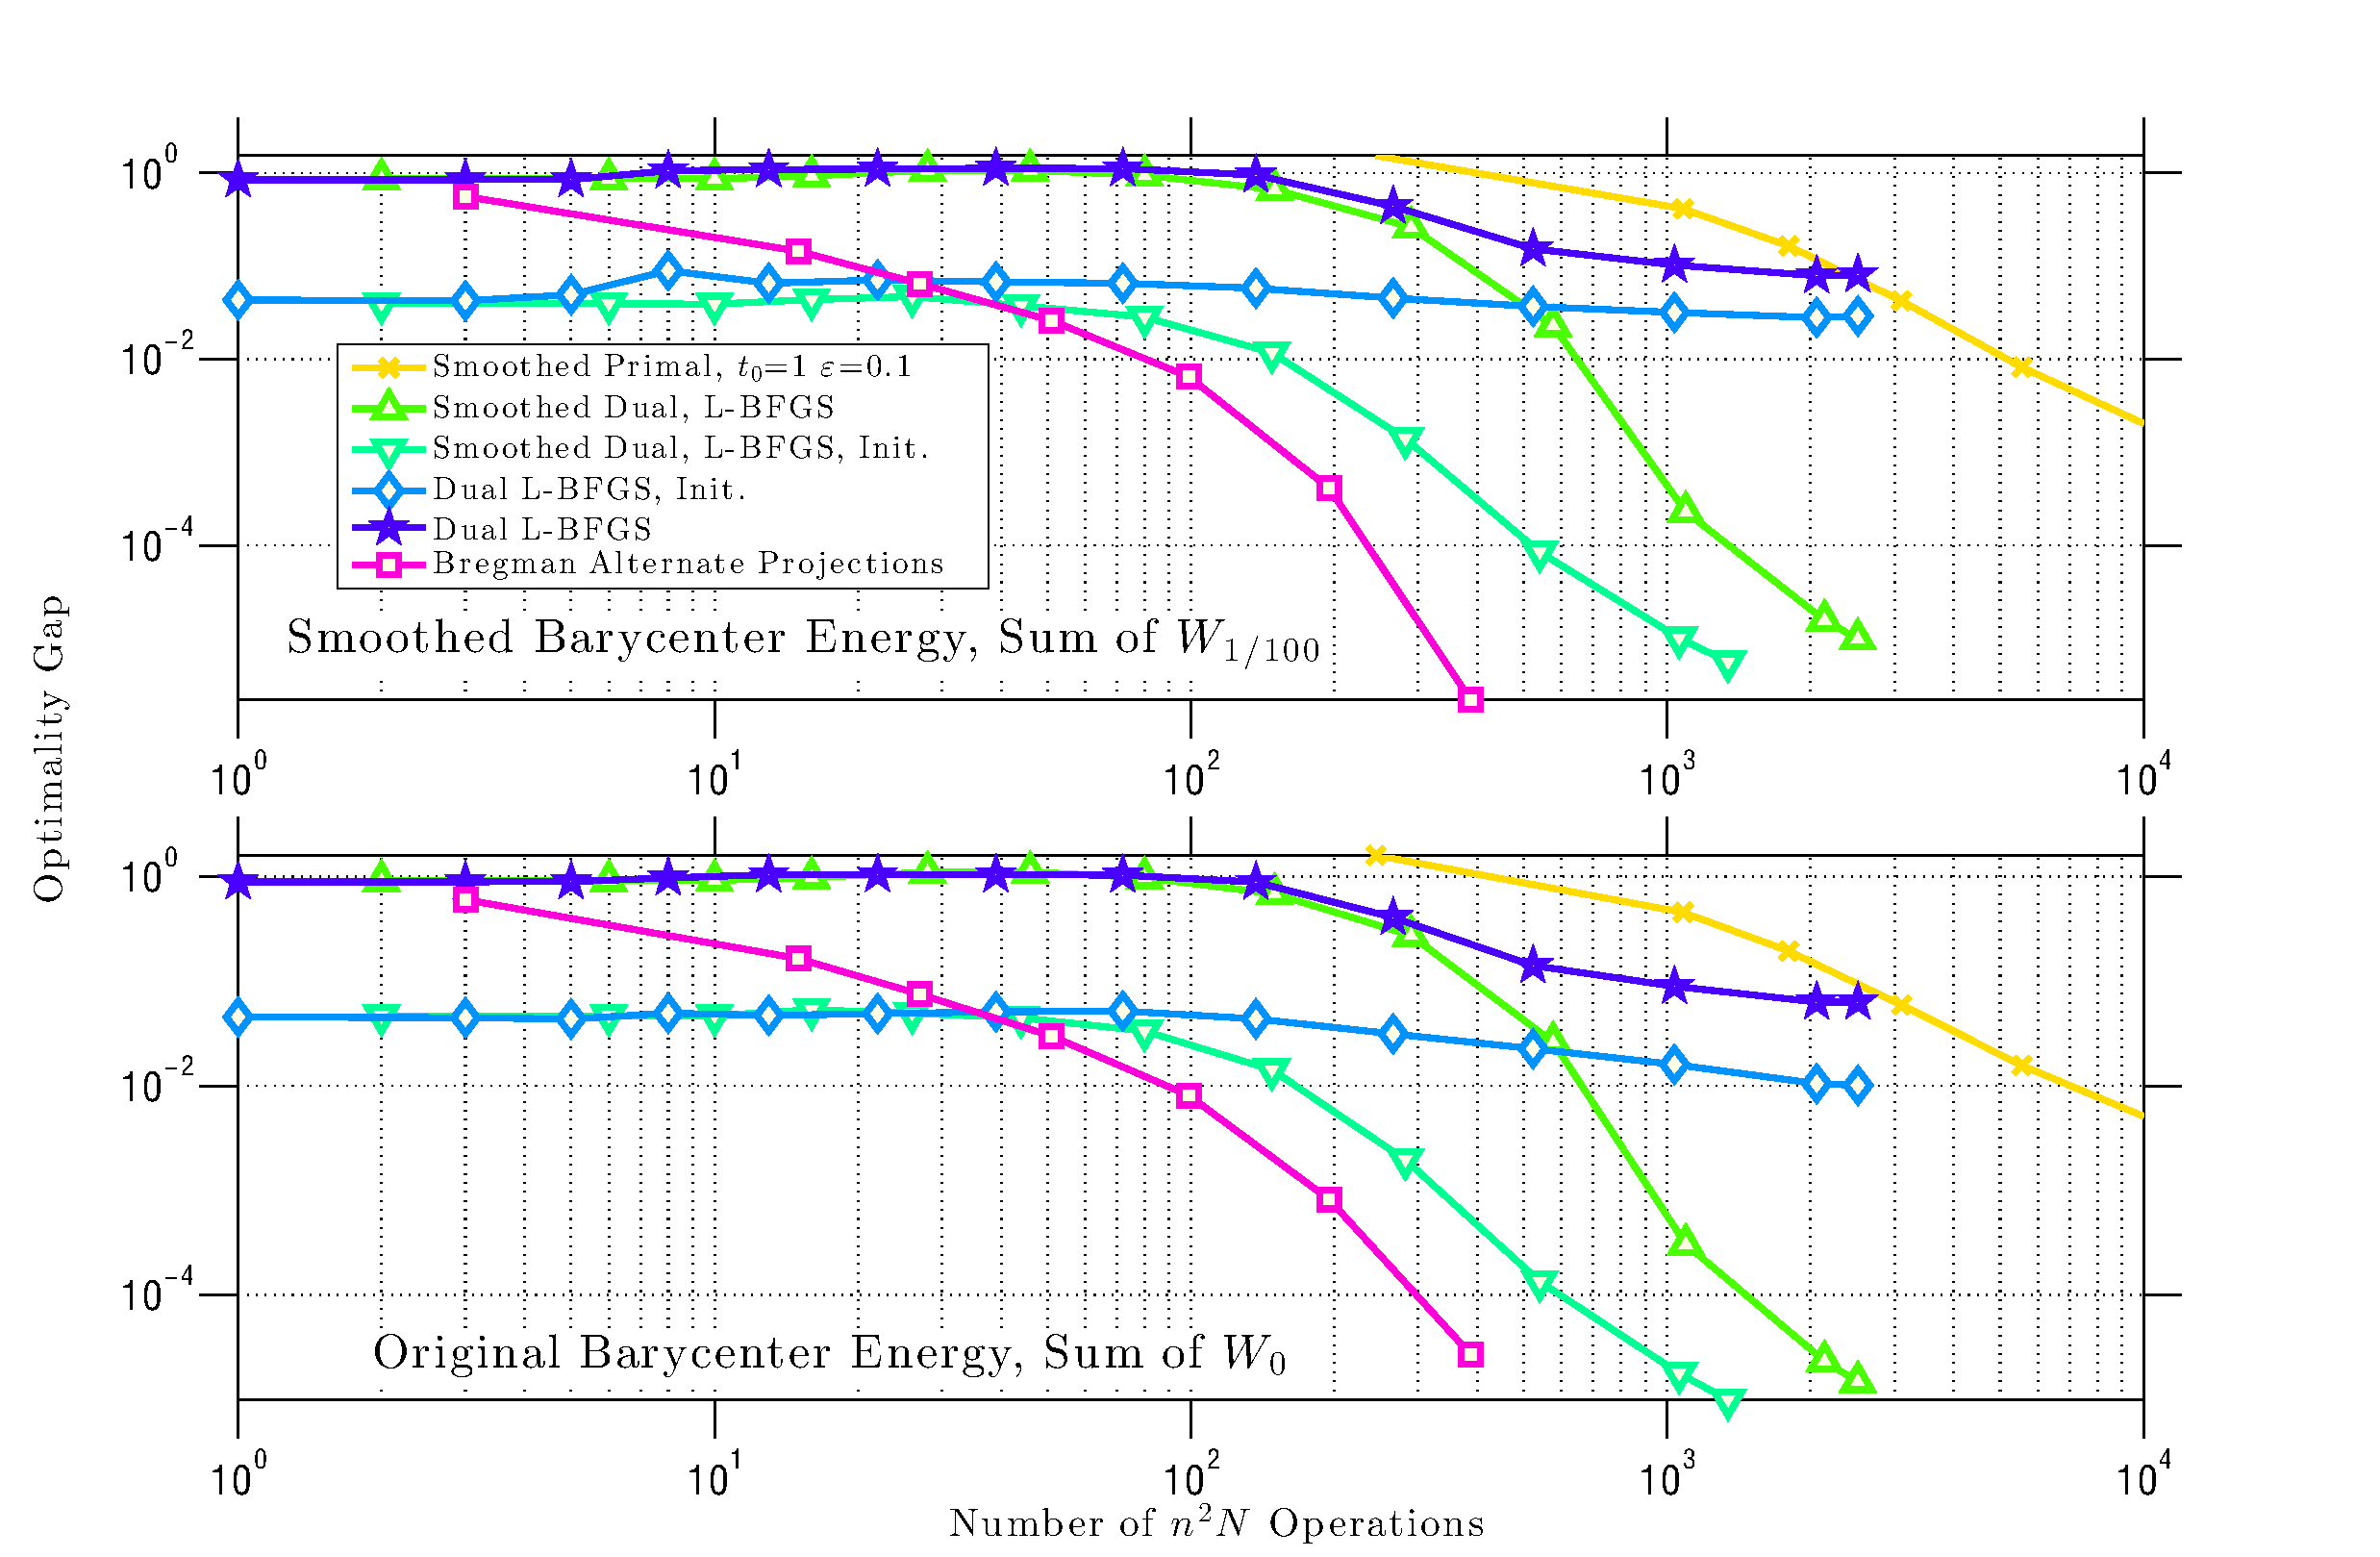
\includegraphics[width=\columnwidth]{experiments.pdf}
	\caption{Number of quadratic operations (matrix vector product or min search in a matrix) \emph{vs.} optimization gap to the smallest possible objective found after running $10^5$ iterations of all algorithms, \emph{log-log} scale. Because the smooth primal/dual approaches optimize a \emph{different} criterion than the dual approach, we plot \emph{both} objectives.  The Smooth dual L-BFGS converges faster in \emph{both} smooth and non-smooth metrics. Note the crucial importance of the initialization proposed in \S\ref{sec:magictrick}.}
\end{figure}


% \begin{figure*}[ht]
% 	\centering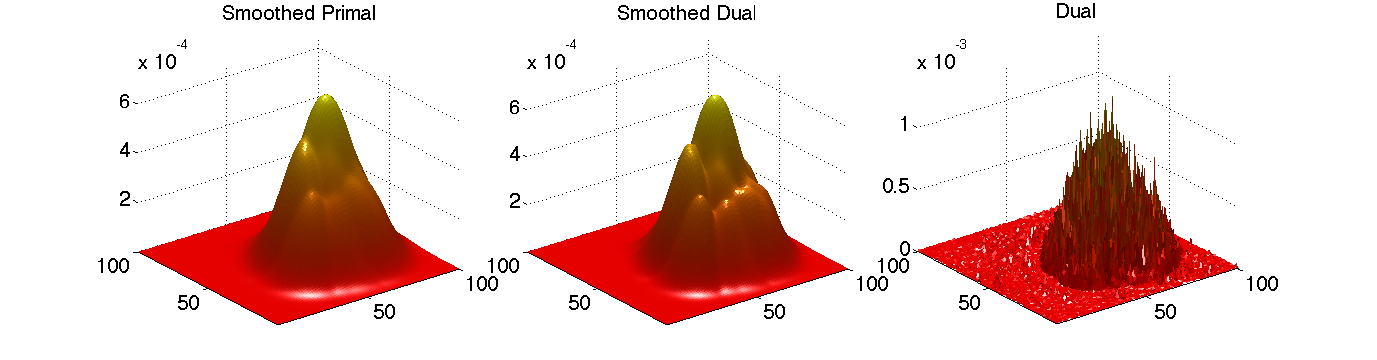
\includegraphics[width=\textwidth]{12barycenters.png}
% 	\caption{Barycenters obtained for the three different techniques using the data described in Figure~\ref{fig:mix} after at most $10^4$ iteration units, each iteration unit being equal to $n^2N$ operations, here $(100\times 100)^2\times 12$.}\label{fig:bar}
% \end{figure*}

\paragraph{Smooth primal first-order descent} \cite[\S5]{cuturi2014fast} proposed to minimize directly Eq.~\eqref{eq-variational-barycenter-discrete} with a regularizer $\ga>0$. That objective can be evaluated by running $N$ Sinkhorn fixed-point iterations in parallel. That objective is differentiable and its gradient is equal to $\ga\sum_k \la_k \log \alpha_k$, where the $\alpha_k$ are the left scalings obtained with that subroutine. A weakness of that approach is that a tolerance $\epsilon$ for the Sinkhorn fixed-point algorithm must be chosen. Convergence for the Sinkhorn algorithm can be measured with a difference in $l_1$ norm (or any other norm) between the row and column marginals of $\diag(\alpha_k)e^{-M/\ga}\diag(\beta_k)$ and the targeted histograms $\p$ and $\q_k$. Setting that tolerance $\epsilon$ to a large value ensures a faster convergence of the subroutine, but would result in noisy gradients which could slow the convergence of the algorithm. Because the smoothed dual approach only relies on closed form expressions we dot not have to take into account such a trade-off.

\paragraph{Iterative Bregman Projections} \cite[Prop. 1]{DBLP:journals/siamsc/BenamouCCNP15} recalls that the computation of the smoothed Wasserstein distance between $p,q$ using the Sinkhorn algorithm can be interpreted as an iterative alternated projection of the $n\times n$ kernel matrix $e^{-M/\ga}$ onto two affine sets, $\{X:X\ones_n=p\}$ and $\{X:X^T\ones_n=q\}$. That projection is understood to be in the Kullack-Leibler divergence sense. More interestingly, the authors also show that the smoothed WBP itself can also be tackled using an iterative alternated projection, cast this time in a space of dimension $ n\times n \times N$. Very much like the original Sinkhorn algorithm, these projections can be computed for a cheap price, by only tracking variables of size $n\times N$. This approach yields an extremely simple, parameter-free, generalization of the Sinkhorn algorithm which can be applied to the WBP.

\paragraph{Smooth dual L-BFGS} 
The dual formulation with variables $(g_1,\cdots,g_N)\in(\RR^n)^N$ of Eq.~\eqref{eq-dual-pbm} can be solved using a constrained L-BFGS solver
At each iteration of that minimization, we can recover a feasible solution $\p$ to the primal problem of Eq.~\eqref{eq-variational-barycenter-discrete} via the primal-dual relation
$\p = \frac{1}{N}\sum_k \nabla H_{\q_k}^*(\tilde g_k).$

\paragraph{Dual $(\ga=0)$ with L-BFGS} This approach amounts to solving directly the (non-differentiable) dual problem described in Eq.~\eqref{eq-dual-pbm} with no regularization, namely $\ga=0$. Subgradients for the Fenchel-Legendre transforms $H_{q_k}^*$ can be obtained in closed form through Proposition~\ref{prop:harddual}. As with the smoothed-dual formulation, we can also obtain a feasible primal solution by averaging subgradients. We follow \cite{Carlier-NumericsBarycenters}'s recommendation to use L-BFGS. The non-smoothness of that energy is challenging: We have observed empirically that a naive subgradient method applied to that problem fails to converge in all examples we have considered, whereas the L-BFGS approach converges, albeit without guarantees.


%, each a mixture of truncated Gaussians on the $100\times 100$ grid, considered to compute the barycenters displayed in Figure
\paragraph{Averaging Truncated Mixtures of Gaussians}
We consider the 12 truncated mixtures of Gaussians introduced in \cite[\S3.2]{DBLP:journals/siamsc/BenamouCCNP15}. To compare computational time, we use $Nn^2$ elementary operations as the computation unit. These $Nn^2$ operations correspond to matrix-matrix products in the smoothed Wasserstein case, and $Nn$ computations of nearest neighbor assignments among $n$ possible neighbors. Note that in both cases (Gaussian matrix product and nearest neighbors under the $L_2$ metric) computations can be accelerated by considering fast Gaussian convolutions and $kd$-trees for fast nearest neighbor search. We do not consider them in this section. We plot the optimality gap w.r.t the optimum of these 4 techniques as a function of the number of computations, by taking as a reference the lowest value attained across all methods. This value is attained, as in \cite{DBLP:journals/siamsc/BenamouCCNP15}, by the iterative Bregman projections approach after 771 iterations (not displayed in our graph). We show these gaps for both the smoothed $(\gamma=1/100)$ and non-smoothed objectives $(\gamma=0)$. We observe that the iterative Bregman approach outperforms all other techniques. The smoothed-dual approach follows closely, notably when initialized with the formula provided in Definition~\ref{def:SI}.

% We also plot the solutions of all 3 algorithms in Figure~\ref{fig:bar} after up to $10^4$ iterations. Because the smoothed-primal and our smoothed-dual approach aim at minimizing the same objective, it is not surprising that their solutions are similar. Note however that with a budget of at most $10^4$ iterations the solution obtained with dual smoothing is more detailed than the one obtained with a primal descent. The right-most figure, obtained following \cite{Carlier-NumericsBarycenters}'s approach, shows that the original Wasserstein barycenter problem formulation, without smoothing, can yield very irregular solutions, as was also observed by the authors themselves in their paper.

